\subsection{Comportamiento Esperado de PageRank}
\label{subsec:exp1}
\begin{LaTeXdescription}
    \item[Objetivo] Ejemplificar el comportamiendo esperado de PageRank.
        Proponemos, a su vez, que el orden obtenido por PageRank ser\'a el mismo
        para cualquier factor de navegaci\'on $\alpha$\footnote{Lo llamamos
        ''factor de navegaci\'on'' al par\'ametro $\alpha$ ya que el mismo
        determina el peso/importancia del grafo/matriz de navegaci\'on $S$
        (definida en la ecuaci\'on \ref{eq:S}, p\'agina \pageref{eq:S}). Se
        puede observar en la definici\'on de $M$ en la p\'agina
        \pageref{eq:M_def} que justamente $\alpha$ define en que porporci\'on
        estar\'an inclu\'idos en $S$ y la matriz de teletransportaic\'on
        uniforme. Llamamos entonces a $\alpha$ factor de navegaci\'on, ya
        que de alguna manera nos indica directamente sin tener que pensar en
        $(1-\alpha)$ en que proporci\'on participa $S$ en $M$, y decimos que
        $S$ es una matriz de navegaci\'on ya que es la matriz que contiene
        los datos de la matriz de conectividad con el inconveniente de los
        dangling nodes resuelto.}, aunque las probabilidades del vector
        resultado (asociadas a cada nodo) cambiar\'an seg\'un este
        par\'ametro.\\

    \item[Proposici\'on] No creemos que haga falta aclarar mucho. Ya se
        present\'o y explic\'o m\'etodo a utilizar. Generaremos un grafo de
        entrada lo suficientemente peque\~no que nos permita calcular a mano el
        resultado de PageRank y explicar el porque de su resultado en base al
        conocimiento del m\'etodo.\\

    \item[M\'etodo de Experimentaci\'on] Realizamos la b\'usqueda
        ''site:uba.ar'' en \emph{Google}\cite{google} y tomamos los primeros 10
        resultados.  Generamos una instancia de entrada utilizando las
        herramientas de la c\'atedra y estos 10 resultados. Por \'ultimo, dada
        esta instancia de prueba, calculamos el \emph{ranking} con el m\'etodo
        PageRank para varios distintos factores de navegaci\'on $\alpha$.\\

    \item[Resultados, an\'alisis y discusi\'on]
\end{LaTeXdescription}

\par En la figura \ref{fig:uba.ar_graph} podemos observar el grafo de
conectividad resultante de los 10 resultados obtenidos por la b\'usqueda
realizada en Google. En el mismo se observan 4 dangling nodes conectados al
grafo: \emph{fvet.uba.ar, ffyb.uba.ar, derecho.uba.ar} y
\emph{videos.agro.uba.ar}, mientras que existen otros dos dangling nodes que no
son alcanzados por ninguno de los nodos del grafo expuesto\footnote{Y por lo
tanto, no los hemos graficado.}: \emph{orga2.exp.dc.uba.ar} y
\emph{iigg.sociales.uba.ar}\footnote{Estos dos sitios que originalmente
aparec\'ian en los primeros 10 resultados de Google al momento de realizar este
experimento, ya no lo hacen m\'as.}.

\begin{figure}[!h]
    \centering
    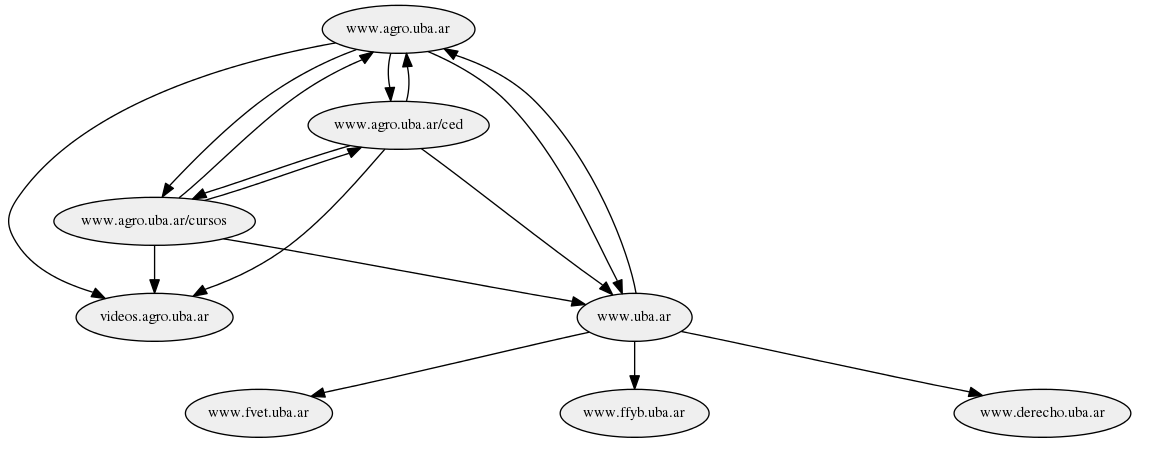
\includegraphics[width=\textwidth]{exp1_conn_graph.png}
    \caption{Grafo de conectividad de la instancia generada con los links
        obtenidos mediante la b\'usqueda en \emph{Google}}
    \label{fig:uba.ar_graph}
\end{figure}

\par Observemos el cuadro \ref{tbl:orden_segun_c} para analizar el orden obtenido.

\begin{table}[hb]
    \centering
    \caption{\'Ordenes obtenidos y sus porcentajes para los resultados obtenidos
        de la b\'usqueda ''site:uba.ar'' en \emph{Google}}
    \label{tbl:orden_segun_c}
    \setlength{\tabcolsep}{3pt}
    \begin{tabular}{|l||r||l||r|r|r|r|r|r|r|r|r|}
        \hline\hline
        \multicolumn{2}{|c||}{Caso particular $\alpha = 0$}&
        \multicolumn{10}{c|}{Casos $0 < \alpha < 1$}\\
        \hline
        Orden/P\'agina & 0 & Orden/P\'agina & 0.1&0.2&0.3&0.4&0.5&0.6&0.7&0.8&0.9\\
        \hline\hline
        derecho.uba.ar& 0.1& 
        agro.uba.ar& 0.103548& 0.107198 & 0.110953 & 0.114823 & 0.118812 &
        0.122929 & 0.127182 & 0.131579 & 0.13613\\
        %
        orga2.exp.dc.uba.ar& 0.1&
        agro.uba.ar/ced& 0.103548& 0.107198 & 0.110953 & 0.114823
        & 0.118812 & 0.122929 & 0.127182 & 0.131579 & 0.13613\\
        %
        agro.uba.ar& 0.1&
        ffyb.uba.ar& 0.103548& 0.107198 & 0.110953 & 0.114823 & 0.118812
        & 0.122929 & 0.127182 & 0.131579 & 0.13613\\
        %
        ffyb.uba.ar& 0.1&
        iigg.sociales.uba.ar& 0.101023& 0.102093 & 0.103212 & 0.104384
        & 0.105611 & 0.106895 & 0.10824& 0.109649 & 0.111127\\
        %
        uba.ar& 0.1&
        orga2.exp.dc.uba.ar& 0.101023& 0.102093 & 0.103212 & 0.104384
        & 0.105611 & 0.106895 & 0.10824& 0.109649 & 0.111127\\
        %
        fvet.uba.ar& 0.1&
        videos.agro.uba.ar& 0.0984973& 0.0969883& 0.0954716& 0.0939457&
        0.0924093& 0.0908605& 0.0892978& 0.0877193& 0.0861231\\
        %
        videos.agro.uba.ar& 0.1&
        agro.uba.ar/cursos& 0.0984973& 0.0969883& 0.0954716& 0.0939457
        & 0.0924093& 0.0908605& 0.0892978& 0.0877193& 0.0861231\\
        %
        iigg.sociales.uba.ar& 0.1&
        fvet.uba.ar& 0.0984973& 0.0969883& 0.0954716& 0.0939457
        & 0.0924093& 0.0908605& 0.0892978& 0.0877193& 0.0861231\\
        %
        agro.uba.ar/cursos& 0.1&
        uba.ar& 0.0959086& 0.0916284& 0.0871502& 0.0824635& 0.0775579&
        0.0724212& 0.0670411& 0.0614038& 0.0554939\\
        %
        agro.uba.ar/ced& 0.1&
        derecho.uba.ar& 0.0959086& 0.0916284& 0.0871502& 0.0824635
        & 0.0775579& 0.0724212& 0.0670411& 0.0614038& 0.0554939\\
        %
        \hline
        Probabilidad Total& 1&
        Probabilidad Total& 0.9999991& 1.0000017& 0.9999982& 1.0000011&
        1.0000017& 1.0000009& 1.0000016& 1.0000005& 1.0000011\\
        \hline\hline
    \end{tabular}
\end{table}

\par Lo primero que debemos se\~nalar es que para obtuvimos siempre el mismo
orden (con distintos valores de convergencia/probabilidad de permanencia) para
$0 < \alpha < 1$; y \'unicamente obtuvimos un orden distinto para $\alpha = 0$.

\par En el caso $\alpha = 0$, esto ocurre pues la matriz $M$ pasa a ser una
matriz tal que $m_{ij} = \rfrac{1}{n}$ para todo $i,j$. Recordemos como era la
definici\'on de $M$ de la ecuaci\'on \ref{eq:M_def}:

\begin{align*}
    M &= \alpha S + (1-\alpha) \frac{1}{n}ee^T \quad\quad\quad \alpha\in\real
    \land \alpha\in\left[0,1\right)\\
    %
    \intertext{Luego, para $\alpha = 0$, tenemos que:}
    M &= 0S + \frac{1}{n}ee^T\\
    M & = \frac{1}{n}ee^T
\end{align*}

\par Por lo tanto, para este caso particular, tenemos una matriz que nos
representa un grafo completo y completamente equiprobable. Es decir, volviendo a
la idea del navegante aleatorio de la secci\'on \ref{sec:introduccion}, que no
importa donde se encuentre el navegante, el mismo se ''mover\'a'' a cualquier
p\'agina web del grafo con la misma probabilidad. As\'i pues, tenemos que en
realidad el navegante deber\'ia pasar la misma cantidad de tiempo en todas las
p\'aginas, lo que explica que el orden devuelto para este caso nos d\'e una
probabilidad de $0.1$ para todas las p\'aginas web/nodos. Claramente aqu\'i el
orden en que PageRank devuelve los sitios se debe a una cuesti\'on del orden de
entrada en cual fueron ingresados los sitios, ya que la coordenada 1 del vector
resultante se corresponde con el sitio 1, la coordenada 2 con el sitio 2, etc.
Si todos los nodos tienen la misma probabilidad, el vector nunca es ordenado
seg\'un las probabilidades y lo que estamos observando es seguramente el orden
en el cual fueron ingresados los nodos.

\par Otra observaci\'on que podemos hacer pasa por la evoluci\'on de los
porcentajes para los distintos $\alpha$ en el intervalo $0.1\dots 0.9$.
Vemos que a medida que aumenta $\alpha$, las probabilidades de los sitios/nodos
que originalmente no eran dangling nodes (y la de aquellos que lo eran, pero
pod\'ian ser alcanzados desde alg\'un nodo) disminuyen, mientras que las de los
dangling nodes completamente inalcanzables en el grafo original
(\emph{orga2.exp.dc.uba.ar} y \emph{iigg.sociales.uba.ar}) aumenta. Lo que
est\'a ocurriendo aqu\'i se debe a la manera en la cual se resolvi\'o el
problema de los dangling nodes. Recordemos que al enfrentar este
escollo\footnote{Gran palabra.} se decidi\'o otorgar la posibilidad de
teletransportaci\'on a cualquier nodo con probabilidad equiprobable a los
dangling nodes. As\'i pues, dado un dangling node $j$, sabemos que $s_{ij} =
\rfrac{1}{n}$ sin importar el $i$. Luego podemos deducir a partir de la
ecuaci\'on \ref{eq:M_def}:

\begin{align*}
    m_{ij} &= \alpha s_{ij} + \dfrac{1-\alpha}{n}\\
           &= \dfrac{\alpha}{n} + \dfrac{1-\alpha}{n}
            \underarrow[=][\uparrow]{$0\leq\alpha<1$} \dfrac{1}{n}\\
    \implies& m_{ij} = \frac{1}{n}\quad\forall j / \text{$j$ dangling node
        inalcanzable}
\end{align*}

\par Es decir, para todo $\alpha$ mayor a 0, vemos que la probabilidad en la
matriz $M$ de los dangling nodes se mantiene inalterada. Esto no ocurre con el
resto de los nodos, que a mayor $\alpha$ ven su valor original de $S$
disminu\'ido y el valor artificial de teletransportaci\'on aumentado. As\'i
pues, pudimos entender porque en el caso de los dangling nodes completamente
aislados del grafo original su probabilidad aumenta conforme aumenta $\alpha$,
mientras que en el caso de los nodos con grado de salida distinto de 0 su
probabilidad disminuye.a mayor $\alpha$. Pero nos queda un caso por analizar: el
de los dangling nodes alcanzables desde el grafo de conectividad.

\par Observemos los valores de 2 dangling nodes alcanzables: \emph{fvet.uba.ar}
y 
